\subsection{Limitations of Perceptrons}

Connectionist neurons, or perceptrons, are limited in the variety of functions they are able to fit. 
When dealing with classification problems, a perceptron can only find a linear separation between any two classes. Irrespective of the neuron's non-linear activation function, the perceptron is regarded as a \emph{linear classifier}. Whether something falls on one side of the decision boundary or the other, is entirely based on applying a linear filter (i.e. $\vec w^{\top} \vec x$). The non-linearity $f(h)$ merely controls the value range of the neuron's response ($\{0,1\}, (-1,+1)$, \ldots) which helps in interpreting the neuron's response.\\

If observations for two different classes are distributed such that one cannot draw a line to separate them, then the two classes
are not linearly separable. In this case the perceptron will fail to find a suitable classification boundary between the two classes.


\begin{frame}\frametitle{Linear classifiers/linear decision boundaries}

Consider the following binary classification problems with $\vec x \in \R^2$.{}

\question{Can you find a line that separates the two classes for each case?}

\begin{figure}[h]
    \centering
	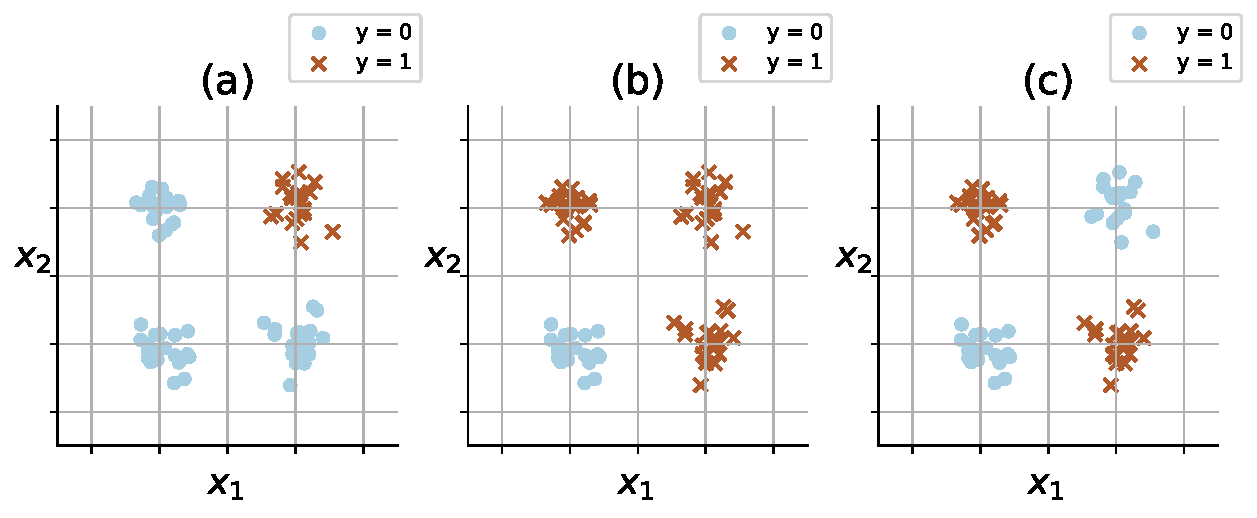
\includegraphics[width=0.8\textwidth]{img/and_or_xor_y}
	\caption{(a) points are classified according to the AND function,
	(b) points are classified according to the OR function,
	(c) points are classified according to the XOR function.
	}
	\label{fig:and_or_xor} 
\end{figure}


\end{frame}

\mode<article>{
In \figureref{fig:and_or_xor}, particularly (a) and (b),
it is possible to draw a line that separates the classes. Therefore, the AND and OR functions are linearly separable.
A perceptron is capable of finding such a separating line. However, this does not apply to the third case, for the XOR function.
It is impossible to find a single line that will separate the classes.\\
The XOR function is not linearly separable.
}

\begin{frame}
\question{Can we solve the XOR problem with multiple perceptrons? How?}

\slidesonly{
\begin{figure}[ht]
     \centering
	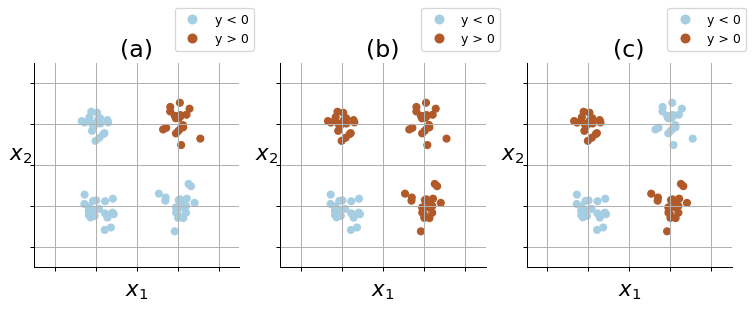
\includegraphics[trim=480 0 0 30, clip, width=0.4\textwidth]{img/and_or_xor_y.png}
	\caption*{A single perceptron can not solve the XOR problem.}
	\label{fig:xor} 
\end{figure}
}

\pause

\notesonly{
- Yes, think of it as a divide and conquer approach. We split the XOR problem into multiple sub-problems. 
A perceptron is used to solve each sub-problem.

If you're familiar with Boolean algebra, you might recognize the following expression for the XOR function:
}

\begin{equation}
\label{eq:xor}
\mathrm{XOR}(x_1, x_2) = 
({\color{magenta}\,{x_1} \; \mathrm{AND} \; \overline{x}_2 \,})
 \;\; \mathrm{OR} \;\; 
({\color{green}\, \overline{x}_1 \; \mathrm{AND} \; x_2 \,})
\end{equation}

\end{frame}

For instance, the first perceptron $S^1_1$ is tasked to separate the bottom-right cloud of points from the rest. 
A second perceptron $S^1_2$ is used to separate the top-left cloud from the rest.
A third perceptron $S^2_1$ will then use the responses from of the first two perceptrons, by responding to ``is only one of the two perceptrons ON?''.

\figref{fig:build_xor} illustrates this approach. One need only recognize that each sub-problem is linearly separable.\\

\begin{frame}
\begin{figure}[ht]
    \centering
	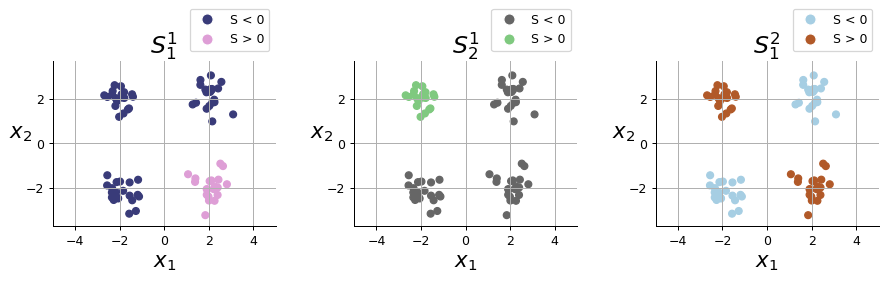
\includegraphics[width=0.9\textwidth]{img/build_xor.png}
	\caption{Solving sub-problems of the XOR problem.}
	\label{fig:build_xor} 
\end{figure}

What we are essentially describing is a Multilayered perceptron (MLP) with an architecture as illustrated in \figref{fig:xor_mlp_arch}. The MLP is made up of an output layer with  a single output neuron $S^2_1$, and one hidden layer with two hidden neurons, $S^1_1$ and $S^2_2$ (the superscript denotes the layer index, the subscript denotes the neuron index within its layer). The terms ``neurons'' and ``nodes'' will be used interchangeably and are treated as synonyms.

\begin{figure}[ht]
    \centering
	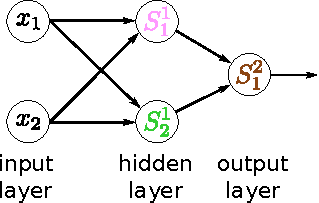
\includegraphics[width=0.5\textwidth]{img/xor_mlp_arch}
	\caption{Simplified MLP architecture for the XOR problem consisting of one hidden layer with two hidden nodes $S^1_1$, $S^1_2$, and one output layer with a single output neuron $S^2_1$}
	\label{fig:xor_mlp_arch} 
\end{figure}

\end{frame}

\clearpage

\section{Feedforward MLP}
\subsection{Navigating through the indices}

\begin{frame}\frametitle{MLP}

\mode<article>{
The nodes in a feedforward neural network form a directed acyclic graph (DAG). There are no connections that feed back to a neuron in an earlier layer. A neuron can only be connected to another neuron that lies in a deeper layer in the network. We will eventually cover neural architectures that allow for feedback connections such as recurrent neural networks.
\figref{fig:mlp_arch} depicts an example MLP architecture.
}

\begin{figure}[ht]
    \centering
	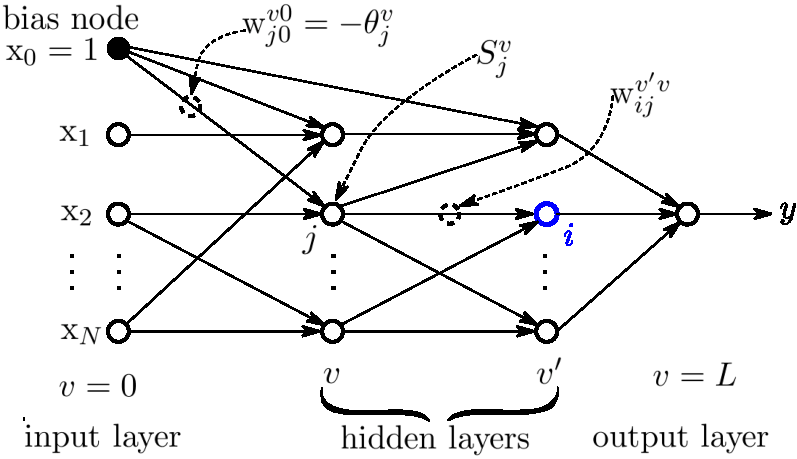
\includegraphics[width=0.7\textwidth]{img/section1_fig14}
	\caption{MLP architecture}
	\label{fig:mlp_arch} 
\end{figure}

\mode<article>{
Each node in the network is a connectionist neuron. This implies that every individual neuron extracts some feature from the ``input'' it receives.
The ``input'' to a neuron can come from the observed data $\vec x$ or it could be the response of another neuron from an earlier layer in the network.
This also implies that \emph{for every neuron} their exists a hyperplane which is represented by some weights $\vec w$ and a bias $\theta$.

$s^v_j$ denotes the \emph{activity} of the neuron $j$-th in layer $v$, while $s^{v'}_i$ denotes the \emph{activity} of the neuron $i$-th in layer $v'$.
$h^v_j$ and $h^{v'}_i$ denotes the \emph{total input} for neuron $(v,j)$ and neuron $(v',i)$, respectively.
The activity $s^{v'}_i$ is obtained by applying a transfer function $f^{v'}_i(\cdot)$ to the total input $h^{v'}_i$ of neuron $(v',i)$:
}

\begin{equation}
s^{v'}_i = f^{v'}_i(h^{v'}_i)
\end{equation}

\mode<article>{
where common choices for $f^v_j(\cdot)$, dpeending on the layer, can be:
\begin{itemize}
\item the identity function: $f^v_j(h) := h$. Often for the input layer, i.e. $s^0_j = f^0_j(h^0_j) = f^0_j(x_j) = x_j$
\item logistic sigmoidal or $\tanh(h)$. Common for hidden neurons and output neurons (for classification tasks).
\end{itemize}

$v$ is a literal that is used to denote a specific layer in the network.\\
$v=0$ describes the \emph{input layer} which holds the observations $\vec x$.\\
$v=L$ describes the \emph{output layer} of the MLP. All the layers in between, if any, are referred to as \emph{hidden layers}. For example, the scalar output of an MLP can be referred to using:


\begin{equation}
y(\vec x;\vec w) = f^L_1(h^L_1)
\end{equation}

$v'$, $v''$ are used to describe layers relative to the current layer $v$. $v'=v+1$ and $v''=v'+1=v+2$ is a very common but this depends on how exactly any two nodes are connected. Therefore, talking about layers $v$, $v'$ and $v''$ needs to be put into the context of the connections between neurons. To elaborate:

$w_{ij}^{v'v}$ measures the strength of the connection \underline{from} $(v,j)$ \underline{to} $(v',i)$. Seeing $v'v$ in the superscript of the weight tells us that the two neurons are directly connected (1 hop).

$w_{j0}^{v0}$ measures the bias $-\theta_{j0}^{v0}$ for neuron $(v,j)$. 

}

\end{frame}

\definecolor{darkgreen}{rgb}{0,0.6,0}
\begin{frame}\frametitle{MLP}

\mode<presentation>{
\begin{figure}[ht]
     \centering
     \savebox{\imagebox}{
	 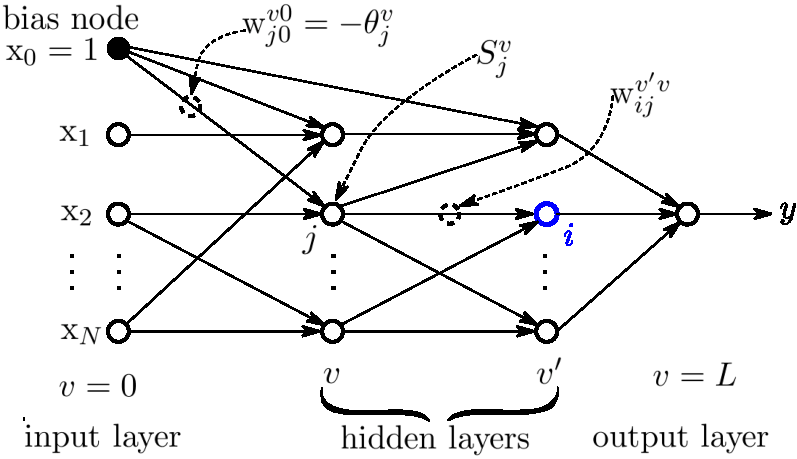
\includegraphics[width=0.6\textwidth]{img/section1_fig14}}%
     \begin{subfigure}[t]{0.6\textwidth}
         \centering
         \usebox{\imagebox}% Place largest image
     \end{subfigure}
     \hfill
     \begin{subfigure}[t]{0.3\textwidth}
         \centering
         \raisebox{\dimexpr.5\ht\imagebox-.5\height}{% Raise smaller image into place
         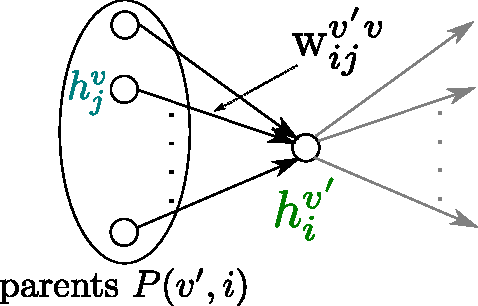
\includegraphics[width=0.9\textwidth]{img/section1_fig20_mini_vdi}
         }
     \end{subfigure}
\end{figure}
}

\mode<article>{

We now look at how this notation describes how a neuron $(v', i)$ processes its input. 

\begin{figure}
    \centering
	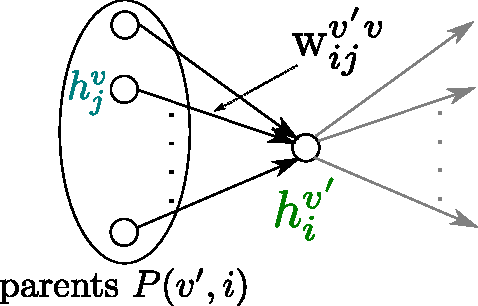
\includegraphics[width=0.4\textwidth]{img/section1_fig20_mini_vdi}
	\caption{Computing the total input for neuron $(v',i)$}
	\label{eq:compute_vdi}
\end{figure}
}

\mode<article>{
The idea is to identify the set of parent nodes $P(v', i)$ that feed input into neuron $(v',i)$. The weighted sum of the parent activations yields the total input ${\color{darkgreen}h^{v'}_i}$
}

\begin{align}
s^{v'}_i = f^{v'}_i(h^{v'}_i) \quad \text{e.g. } s^{v'}_i = f^{v'}_i\big(\sum_{j=0}^{N_{v}} w_{ij}^{v'v} s^v_j\big)
\end{align}

\end{frame}
